\documentclass[12pt]{article}
\usepackage[utf8]{inputenc}

\usepackage{enumitem}
\usepackage[margin=2cm]{geometry}

\usepackage{amsmath, amsfonts, amssymb}
\usepackage{graphicx}
\usepackage{tikz}
\usepackage{pgfplots}
\usepackage{multicol}

\usepackage{comment}
\usepackage{url}
\usepackage{calc}
\usepackage{subcaption}

\usepackage{array}

\setlength\parindent{0pt}

\usepackage{fancyhdr}
\pagestyle{fancy}
\fancyhf{}
\renewcommand{\headrulewidth}{2pt}
\renewcommand{\footrulewidth}{0pt}
\rfoot{\thepage}
\lhead{\textsc{Math} 244}
\chead{\textsc{Homework 5}}
\rhead{Fall 2023}

\pgfplotsset{compat=1.16}

% MATH commands
\newcommand{\ga}{\left\langle}
\newcommand{\da}{\right\rangle}
\newcommand{\oa}{\left\lbrace}
\newcommand{\fa}{\right\rbrace}
\newcommand{\oc}{\left[}
\newcommand{\fc}{\right]}
\newcommand{\op}{\left(}
\newcommand{\fp}{\right)}

\newcommand{\bi}{\mathbf{i}}
\newcommand{\bj}{\mathbf{j}}
\newcommand{\bk}{\mathbf{k}}
\newcommand{\bF}{\mathbf{F}}

\newcommand{\ra}{\rightarrow}
\newcommand{\Ra}{\Rightarrow}

\newcommand{\sech}{\mathrm{sech}\,}
\newcommand{\csch}{\mathrm{csch}\,}
\newcommand{\curl}{\mathrm{curl}\,}
\newcommand{\dive}{\mathrm{div}\,}

\newcommand{\ve}{\varepsilon}
\newcommand{\spc}{\vspace*{0.5cm}}

\DeclareMathOperator{\Ran}{Ran}
\DeclareMathOperator{\Dom}{Dom}

\newcommand{\exo}[3]{\noindent\textcolor{red}{\fbox{\textbf{Section {#1}, Problem {#2}}}\hrulefill   \textbf{({#3} Pts})}\vspace*{10pt}}

\begin{document}
\thispagestyle{empty}
	\noindent \hrulefill \newline
	MATH-244 \hfill Pierre-Olivier Paris{\'e}\newline
	Homework 5 Solutions \hfill Fall 2023\newline \vspace*{-0.7cm}
	
	\noindent\hrulefill
	
	\spc
	
	\exo{15.6}{36}{10}

	Based on the bounds in each integral, we can describe $E$ as followed:
		\begin{align*}
		E = \{ (x, y ,z) \, : \, 0 \leq x \leq z , \, 0 \leq y \leq 1 , \, y \leq z \leq 1 \}
		\end{align*} 
	The solid is described as a Type 2 and is illustrated in the picture below. The solid is enclosed by the blue, yellow, and green planes.
	\begin{center}
		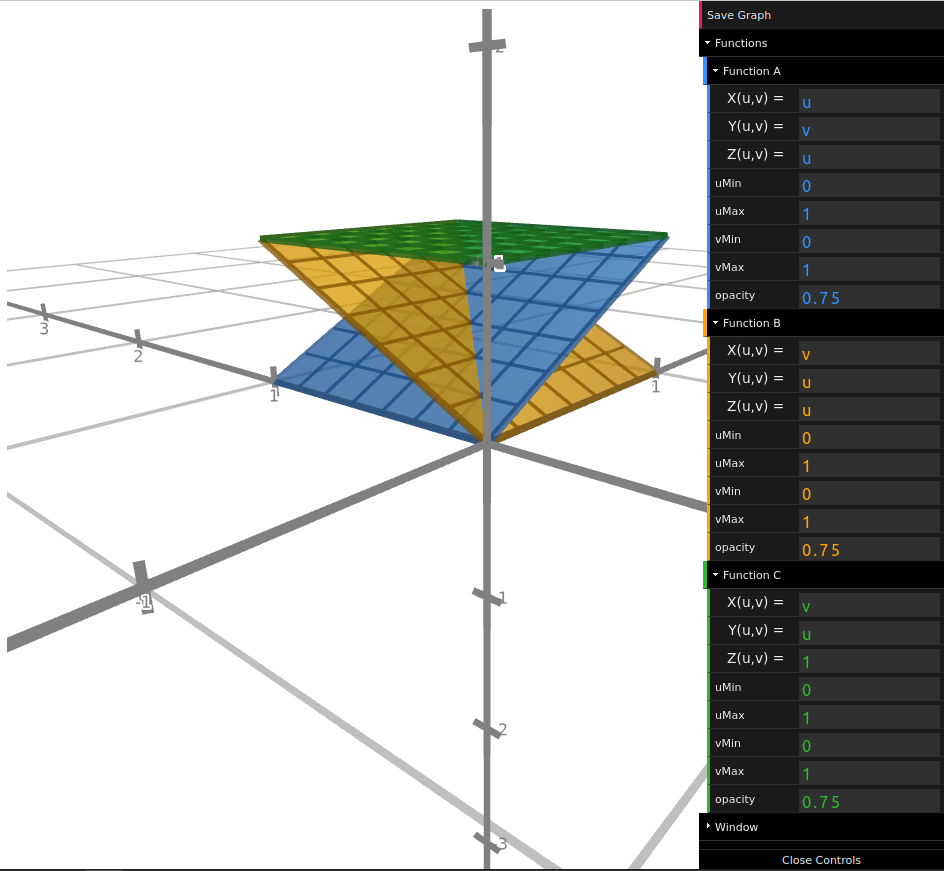
\includegraphics[scale=0.2]{Solid-15-6-exo36.png}
	\end{center}

	We will describe it as a Type 3, so we need to bound the $y$ values. The $y$ values will be bounded by $y = 0$ and $y = z$ (the plane in yellow in the picture). Then the shadow of the solid in the $XZ$-plane will be a triangular region that can be described as followed: 
		\begin{align*}
		D = \{ (x, z) \, : \, 0 \leq x \leq z , \, 0 \leq z \leq 1 \} .
		\end{align*} 
	Therefore, the integral can be rewritten as
		\begin{align*}
		\int_0^1 \int_0^z \int_0^z f (x, y, z) \, dy dx dz .
		\end{align*}

	We can also describe is as a Type 1. But we have to split into two integrals because the bounds for the $z$ values will change (from the blue plane to the yellow plane). The shadow of the object in the $XY$-plane is a square $[0, 1] \times [0, 1]$. The two planes $x = z$ and $y = z$ meets exactly when $y = x$. We will therefore divide the square $[0, 1] \times [0 , 1]$ along the line $y =x$ into two rectangular regions, call them $R_1$, and $R_2$. We have
		\begin{align*}
		R_1 = \{ (x, y) \, : \, 0 \leq x \leq 1 , 0 \leq y \leq x \} \quad \text{ and } \quad R_2 = \{ (x, y) \, : \, 0 \leq x \leq 1 , x \leq y \leq 1 \} .
		\end{align*} 
	On $R_1$, we have $x \leq z \leq 1$. On $R_2$, we have $y \leq z \leq 1$. Therefore, the integral takes the following form:
		\begin{align*}
		\int_0^1 \int_0^x \int_x^1 f (x, y, z) \, dz dy dx + \int_0^1 \int_x^1 \int_y^1 f (x, y, z) \, dz dy dx .
		\end{align*}
	
	Notice that we could change the order of $dx dz$ to $dz dx$ and $dy dx$ to $dx dy$ respectively.

	\newpage
	
	\exo{15.7}{10}{10}

	\begin{enumerate}[label=\alph*)]
		\item We set $x = r \cos \theta$ and $y = r \sin \theta$ and $z = z$. Therefore,
			\begin{align*}
			2x^2 + 2y^2 - z^2 = 2 r^2 \cos^2 (\theta ) + 2 r^2 \sin^2 (\theta ) - z^2 = 2r^2 - z^2
			\end{align*} 
		and the equation is $2r^2 - z^2 = 4$.
		\item We set $x = r \cos \theta$, $y = r \sin \theta$, and $z = z$. Therefore,
			\begin{align*}
			2x - y + z = 2r \cos \theta - r \sin \theta + z = r (2 \cos \theta - \sin \theta ) + z . 
			\end{align*} 
		The equation becomes $r (2 \cos \theta - \sin \theta ) + z = 1$. 
	\end{enumerate}

	\exo{15.7}{18}{10}

	The solid $E$ can be described easily as a type 1. The $z$-values are bounded below by $z = x^2 + y^2$ and above by $z = 4$. The shadow created in the $xy$-plane is a circular region bounded by the circle $x^2 + y^2 = 4$ of radius $2$. Therefore, using polar coordinates in the $xy$-plane, we have
		\begin{align*}
		\iiint_E z \, dV = \int_0^{2\pi} \int_0^2 \int_{r^2}^4 z \, dz \, r dr d\theta &= \int_0^{2\pi} \int_0^2 \frac{16 - r^4}{2} \, r dr d \theta \\
		&= \Big( \int_0^2 8r - \frac{r^5}{2} \, dr \Big) \Big( \int_0^{2\pi} \, d \theta \Big) \\
		&= (32/ 3) (2\pi ) \\
		&= \frac{64 \pi}{3} . \tag*{$\triangle$}
		\end{align*} 


	\exo{15.7}{22}{10}

	We will describe the solid enclosed by the sphere and the cylinder as a type 1. This is because the $z$-values are restricted by the sphere in the following way:
		\begin{align*}
		-\sqrt{4 - x^2 - y^2} \leq z \leq \sqrt{4 - x^2 - y^2} .
		\end{align*}
	The shadow in the $xy$-plane will simply be the inside of the circle, that is a circular shape bounded by the circle $x^2 + y^2 = 1$. Therefore, in cylindrical coordinates:
		\begin{align*}
		E = \{ (r, \theta , z) \, : \, 0 \leq r \leq 1 , 0 \leq \theta \leq 2\pi , -\sqrt{4 - x^2 - y^2} \leq z \leq \sqrt{4 - x^2 - y^2} \} .
		\end{align*}

	The volume is given by the triple integral of $1$ over the solid $E$. Therefore,
		\begin{align*}
		\mathrm{Vol} (E) = \iiint_E 1 \, dV &= \int_0^{2 \pi} \int_0^1 \int_{-\sqrt{4 - r^2}}^{\sqrt{4 - r^2}} \, dz r dr d\theta \\
		&= \int_0^{2\pi} \int_0^1 2 r \sqrt{4 - r^2} \, dr d\theta \\ 
		&= \Big( \int_0^1 2r \sqrt{4 - r^2} \, dr \Big) \Big( \int_0^{2\pi} \, d\theta \Big) \\
		&= \Big( \int_3^4 \sqrt{u} \, du \Big) 2\pi \\
		&= \Big( \frac{16}{3} - 2 \sqrt{3} \Big) 2\pi . \tag*{$\triangle$}
		\end{align*}

	\exo{15.7}{30}{10}
	
	From the bounds in the integrals, we see that
		\begin{align*}
		E = \{ (x, y, z) \, : \, -3 \leq x \leq 3 , \, 0 \leq y \leq \sqrt{9 - x^2} , \, 0 \leq z \leq 9 - x^2 - y^2 \} .
		\end{align*}
	The region $D$ described by $(x, y)$ such that $-3 \leq x \leq 3$ and $0 \leq y \leq \sqrt{9 - x^2}$ is in fact a circular region bounded by the circle $x^2 + y^2 = 9$. With this observation and by using cylindrical coordinates, we see that 
		\begin{align*}
		E = \{ (r, \theta , z ) \, : \, 0 \leq r \leq 3 , 0 \leq \theta \leq  \pi , 0 \leq z \leq 9 - r^2 \} .
		\end{align*} 
	Therefore, 
		\begin{align*}
		\iiint_E \sqrt{x^2 + y^2} \, dV = \int_0^{2\pi} \int_0^3 \int_0^{9 - r^2} r \, dz r dr \theta &= \int_0^{2\pi} \int_0^3 r^2 (9 - r^2) \, dr d\theta \\
		&= \Big( \int_0^3 9r^2 - r^4 \, dr \Big) \Big( \int_0^{2\pi} \, d\theta \Big) \\
		&= \frac{162 \pi}{5} \tag*{$\triangle$} 
		\end{align*} 

\end{document}